%\documentclass{article}
%\usepackage{graphicx} % Required for inserting images
%\usepackage{amsmath}

\documentclass[a4paper, notitlepage,12pt]{article}
\usepackage[utf8]{inputenc}
\linespread{1.5}
\usepackage{graphicx}
\usepackage{xcolor}
\usepackage{appendix}
\usepackage{natbib}
%\usepackage{geometry}
%\geometry{a4paper, textwidth=  15cm, textheight= 24cm, centering }

\usepackage[left=1in, right=1in, top=1in, bottom=1in]{geometry}

\usepackage{placeins}
\usepackage{booktabs}
\usepackage{hyperref}
\usepackage{setspace}
\usepackage{subfiles}
\usepackage{lscape}

\usepackage{soul}

\usepackage{array}
\usepackage{graphicx} % Required for the \resizebox command
\usepackage{booktabs} % Optional: for the \cmidrule and \midrule
\usepackage{adjustbox}

\usepackage{amssymb}
\usepackage{amsfonts}
\usepackage{amsmath}
\usepackage{amsthm}
\usepackage{caption,subcaption}

\usepackage{soul}
\definecolor{highlightcolor}{RGB}{255,255,150}
\sethlcolor{highlightcolor}

\usepackage{tabularx}
\usepackage{pdflscape}

\newcommand{\plim}{\operatorname{plim}}
%\newcommand{\E}{\mathbb{E}}
\newtheorem{theorem}{Theorem}

\title{\textbf{Measuring the Financial Cycle: A Dynamic Factor Model Approach}}
\author{Daniel Abreu* and  
Ivan De Lorenzo Buratta**}
\date{\today }
% \title{\textbf{FINANCIAL CYCLE}}
% \author{Daniel Abreu$^{a}$~ and  
% Ivan De Lorenzo Buratta$^{b}$ \\
%  $^{a}${\small {}Banco de Portugal}\\		$^{b}${\small {}XX}}
% \date{\today }

\begin{document}

\maketitle
 \begin{abstract}
 \noindent 
 This paper proposes a novel approach to measuring the financial cycle using a dynamic factor model (DFM) that synthesizes information from key financial indicators. We construct country-specific financial cycle indicators for a sample of European economies and show that they provide a coherent measure of cyclical systemic risk. A central contribution of the paper is the evaluation of the indicator in a pseudo real-time, out-of-sample setting. We find that it delivers economically meaningful early-warning signals of financial crises, with the estimated one-year-ahead probability of a crisis increasing markedly—more than doubling—in the run-up to the Global Financial Crisis. Our empirical results further show that the proposed indicator identifies the key drivers of financial cycle fluctuations and provides a statistically grounded framework for defining a neutral level of systemic risk. These features make the approach a useful tool for monitoring cyclical systemic risk and for informing macroprudential policy.


\vspace{0.25cm}

\textbf{JEL codes}: C54; E44; E58; G01.

\textbf{Keywords}: Financial cycle; Dynamic factor model; cyclical systemic risk.
 
 \end{abstract}


\vspace{0.25cm}

\noindent
\begin{footnotesize}


  { \color{blue} 
  \noindent * XXX. E-mail: YYY
  
  \noindent ** Prometeia. E-mail: ivan.delorenzoburatta@prometeia.com 
  
  \noindent Acknowledgments: We should thank here BdP people who read the work/attended our presentation. Same for the ECB task force - you presented twice if I recall correctly. Example:
    We thank XXX, YYY, ZZZ and the participants of the XXX Workshop for the helpful comments. The views expressed in this article are those of the authors. Any errors and mistakes are ours. Competing interests: the authors declare none.}
\end{footnotesize}

\newpage

\section{Introduction \label{Intro}}\input{1. INTRO}
\section{Data}\subsection{Variable selection}

\paragraph{Definitions.} 
\citet{borio2014financial} defines the financial cycle as ``self-reinforcing interactions between perceptions of value and risk, attitudes towards risk, and financing constraints, which translate into booms followed by busts." This definition highlights that the financial cycle is characterised by joint fluctuations in credit, asset prices, and leverage that can become disconnected from underlying fundamentals. As financial imbalances accumulate over time, cyclical systemic risk increases, raising the likelihood of severe downturns and banking crises.

Measuring the financial cycle therefore requires selecting variables that capture both the build-up of financial imbalances and their potential materialisation. In this paper, we focus on four key dimensions: credit, asset prices, indebtedness, and financial conditions. These dimensions are chosen based on their established role in the literature as core components of cyclical systemic risk and their relevance for early-warning analysis.

To preserve interpretability and ensure a transparent link between the estimated factor and its underlying drivers, we deliberately restrict the analysis to a parsimonious set of variables within each dimension. This approach facilitates the economic interpretation of the financial cycle indicator while retaining the key information needed to capture its dynamics.

\paragraph{Credit.}  

The central role of credit in the financial cycle is well established in both theoretical and empirical work. Early contributions by \citet{fisher1933debt} and \citet{minsky1977financial} highlight the role of credit cycles in generating and amplifying macroeconomic instability, while subsequent work shows how credit acts as a propagation mechanism for shocks \citep{bernanke1983non, gertler1988financial}. This mechanism is formalised in the financial accelerator framework of \citet{bernanke1999financial}, which emphasises the endogenous amplification of shocks through credit market conditions. Empirically, credit aggregates have been shown to be among the most reliable predictors of systemic banking crises \citep{schularick2012credit}.

To capture these dynamics, we include two measures of credit: credit to non-financial corporations and credit to households (including non-profit institutions). This distinction allows us to account for differences in borrowing behaviour across sectors, which may have distinct implications for the build-up of cyclical systemic risk. Both series are constructed from the total stock of credit to the private non-financial sector, covering all sources of financing including domestic banks, non-bank financial institutions, non-financial corporations, and cross-border lending. As such, the indicator provides a comprehensive measure of credit developments in the economy.

\paragraph{Asset prices.}  

Asset prices play a central role in the financial cycle, both as indicators of financial imbalances and as channels through which shocks are amplified. In particular, increases in asset prices can relax borrowing constraints and support credit expansion, while subsequent declines can trigger adverse feedback loops by reducing collateral values \citep{kiyotaki1997credit}. Empirically, asset price dynamics—especially in housing markets—are closely associated with the build-up and materialisation of systemic risk \citep{jorda2015leveraged, claessens2012business}. House prices, in particular, have been shown to be strong predictors of banking crises, while equity prices often peak prior to crisis episodes \citep{mian2014explains, reinhart2013banking}.

To capture these dynamics, we include both house price and share price indices. The house price index reflects inflation-adjusted transaction prices of residential property, providing a measure of developments in real estate markets that are closely linked to credit conditions. Share price indices capture the prices of publicly traded equities, aggregated from daily closing values, and provide forward-looking information on market valuations and risk sentiment.

\paragraph{Indebtedness.} 

While credit captures the expansion of financing over the financial cycle, indebtedness reflects the accumulation of debt and the associated vulnerabilities in the economy. High levels of leverage increase the sensitivity of households, firms, and financial intermediaries to adverse shocks, as declines in income or asset prices can impair debt servicing capacity and amplify financial distress \citep{adrian2010liquidity, brunnermeier2009market}. As a result, elevated indebtedness is a key determinant of the severity of downturns and the materialisation of systemic risk.

To capture these dynamics, we include two complementary indicators: the credit-to-GDP ratio and the debt service ratio (DSR). The credit-to-GDP ratio provides a measure of the stock of debt relative to the size of the economy and is widely used as an indicator of systemic risk, with well-documented early-warning properties for banking crises \citep{aikman2015curbing}. The DSR captures the share of income devoted to debt servicing, providing a direct measure of repayment burden and financial stress faced by households and non-financial corporations. Together, these variables capture both the level and the sustainability of indebtedness over the financial cycle.

\paragraph{Financial conditions.}

Financial conditions capture the pricing of risk and the level of risk appetite in financial markets, both of which are central to the financial cycle. We proxy these conditions using the spread between each country’s 10-year sovereign bond yield and that of Germany, which serves as a benchmark reflecting low credit risk within the European context. Changes in sovereign spreads provide information on shifts in perceived risk and financing conditions, as increases in risk premia tend to coincide with periods of financial stress.

This measure is closely related to indicators used in financial stress indices \citep{hubrich2015financial}, which distinguish periods of low risk appetite from episodes of heightened uncertainty. Moreover, sovereign bond spreads are informative about broader financial conditions, as movements in sovereign risk premia are often mirrored in borrowing costs for households, firms, and financial intermediaries. Including this variable therefore enhances the ability of the indicator to capture the materialisation of systemic risk, complementing other variables that primarily reflect its build-up.

\subsection{Variable treatment}

\paragraph{Stationarity.} 

An underlying assumption of dynamic factor models is that the data are covariance stationary. To satisfy this requirement, all variables, except the government bond spread, are transformed into 2-year growth rates, while the bond spread is expressed in 2-year differences. These transformations are guided by unit root tests and case-by-case judgement.

The choice of 2-year growth rates reflects the medium-term nature of the financial cycle and is supported by evidence that longer-horizon transformations exhibit stronger early-warning properties for systemic banking crises \citep{lang2019anticipating}. By focusing on medium-term dynamics, this approach captures the gradual build-up of financial imbalances that precede crisis episodes.

Importantly, this methodology analyses cycles in growth rates rather than relying on gap measures, such as the credit-to-GDP gap, which extract cyclical components from time series levels. In line with \citet{schuler2020financial} and \citet{lang2019anticipating}, this avoids the spurious cycles and endpoint biases often associated with filtering techniques \citep{schuler2018detrending}, providing a more robust representation of financial cycle dynamics.

\paragraph{Low-Frequency Movements.} 

To isolate the cyclical components of the variables, low-frequency movements are removed from the data. Long-term trends often reflect structural changes and can obscure medium-term fluctuations relevant for the financial cycle. As emphasized by \citet{stock2016dynamic}, removing these low-frequency components is essential for distinguishing persistent trends from cyclical dynamics in macroeconomic time series.

This is particularly relevant in the European context, where greater financial integration and the introduction of the euro have significantly influenced long-term financial dynamics and contributed to the synchronization of financial cycles across countries \citep{jorda2018global, aikman2015curbing}. In addition, the post-GFC period has been marked by significant institutional changes that have reshaped the functioning of financial markets. Accounting for these low-frequency movements is therefore important to avoid conflating structural trends with cyclical fluctuations.

In line with this approach, we apply a filtering method to extract medium-term dynamics \citep{drehmann2012characterising, schuler2020financial}. Specifically, we use the Butterworth filter proposed by \citet{pollock2000trend}, which offers greater flexibility than the Hodrick–Prescott (HP) filter in capturing time-varying trends.

We focus on cycles with periodicities between 4 and 25 years. Frequencies longer than 25 years are removed to exclude low-frequency trends, while fluctuations with periodicities shorter than 4 years are filtered out to reduce high-frequency noise. This approach allows us to isolate medium-term financial cycle dynamics in a consistent and robust manner.

\paragraph{Standardization.}  

All variables are standardized to have zero mean and unit variance. This is a standard step in dynamic factor models, as the estimated factor is sensitive to the scale of the variables. Standardization ensures comparability across variables and allows the resulting financial cycle indicator to be interpreted in terms of deviations from its historical average. In this framework, large positive or negative values of the indicator reflect significant departures from typical conditions and can be interpreted as signals of financial imbalances.

\subsection{Descriptive statistics}

\paragraph{Sample.} Our sample consists of quarterly data for 10 European countries: Sweden (SE), Italy (IT), France (FR), Germany (DE), Belgium (BE), the Netherlands (NL), Finland (FI), the United Kingdom (GB), Portugal (PT), and Spain (ES). The dataset spans from 1995 Q3 to 2024 Q3. The country selection balances sample length with data availability across countries. Our focus on European countries reflects their exposure to similar economic shocks and similar institutional frameworks, enabling more meaningful comparisons. In the following sections, we construct the financial cycle indicator for each country and present the results by examining the distribution of the indicator across the sample.

\paragraph{Descriptive statistics.}  
  
Table \ref{sum_st} reports summary statistics for the selected variables, expressed in 2-year growth rates, except for bond spreads, which are presented in 2-year differences. The results reveal substantial heterogeneity across countries and across types of financial indicators.

Credit to non-financial corporations shows moderate average growth across countries, ranging from 7.3\% in Italy to 14.4\% in Spain, with relatively limited dispersion. In contrast, credit to households grows more strongly and is more volatile, particularly in Portugal (17.2\%), Spain (13.9\%), and Sweden (13.7\%).

Asset price dynamics display greater cross-country variation. House prices record positive average growth in most countries, with higher values in Sweden (9.2\%) and the United Kingdom (8.1\%), while Italy stands out with a negative average growth rate (-0.5\%). Equity prices exhibit robust growth across all countries, reaching 25.5\% in Finland and 22.6\% in Sweden, but with substantial volatility.

Indicators of indebtedness show more moderate dynamics. Debt service ratios display near-zero average growth across countries, ranging from -1.7\% in Germany to 2.1\% in Belgium. By contrast, credit-to-GDP ratios increase more noticeably in countries such as Spain (5.0\%), Belgium (4.3\%), Portugal (3.8\%), and Sweden (4.2\%), indicating a gradual accumulation of leverage over the sample period.

Finally, sovereign bond spreads generally decline over the sample period, particularly in Portugal (-21\%), Sweden (-18\%), and Spain (-17\%). As Germany serves as the benchmark for the spread measure, it is not directly comparable to other countries in this dimension. Variability in spreads is highest in Portugal, reflecting the pronounced fluctuations observed during the sovereign debt crisis.

\begin{table}[htbp]
\centering
\caption{Summary statistics}
\label{sum_st}

\resizebox{\textwidth}{!}{%
\begin{tabular}{l *{14}{r}}
\toprule
& \multicolumn{2}{c}{\shortstack{Credit\\NFC}} 
& \multicolumn{2}{c}{\shortstack{Credit\\Households}} 
& \multicolumn{2}{c}{\shortstack{House\\prices}} 
& \multicolumn{2}{c}{\shortstack{Share\\prices}} 
& \multicolumn{2}{c}{DSR} 
& \multicolumn{2}{c}{\shortstack{Credit-to-\\GDP}} 
& \multicolumn{2}{c}{\shortstack{Bond\\spread}} \\
\cmidrule(lr){2-3}\cmidrule(lr){4-5}\cmidrule(lr){6-7}\cmidrule(lr){8-9}\cmidrule(lr){10-11}\cmidrule(lr){12-13}\cmidrule(lr){14-15}
\textbf{Country} 
& \textbf{mean} & \textbf{sd}
& \textbf{mean} & \textbf{sd}
& \textbf{mean} & \textbf{sd}
& \textbf{mean} & \textbf{sd}
& \textbf{mean} & \textbf{sd}
& \textbf{mean} & \textbf{sd}
& \textbf{mean} & \textbf{sd} \\
\midrule
BE & 13.1\% & 11.1\% & 11.1\% & 5.1\%  & 5.0\%  & 5.4\%  & 13.4\% & 33.4\% & 2.1\%  & 7.8\%  & 4.3\% & 7.9\%  & -0.02 & 0.48 \\
DE & 7.4\%  & 6.8\%  & 5.4\%  & 5.3\%  & 1.1\%  & 7.4\%  & 13.0\% & 30.9\% & -1.7\% & 4.0\%  & 0.7\% & 5.1\%  & -0.32 & 1.07 \\
ES & 14.4\% & 21.2\% & 13.9\% & 19.3\% & 4.9\%  & 14.3\% & 13.7\% & 38.5\% & 0.3\%  & 13.6\% & 5.0\% & 13.6\% & -0.17 & 1.33 \\
FI & 9.6\%  & 8.2\%  & 12.3\% & 9.6\%  & 3.7\%  & 8.2\%  & 25.5\% & 63.8\% & 0.1\%  & 10.4\% & 2.2\% & 7.2\%  & -0.11 & 0.50 \\
FR & 9.3\%  & 4.7\%  & 11.0\% & 5.4\%  & 5.6\%  & 10.2\% & 14.4\% & 30.9\% & 0.9\%  & 5.9\%  & 3.5\% & 4.7\%  & 0.01  & 0.31 \\
GB & 10.7\% & 10.8\% & 11.4\% & 8.1\%  & 8.1\%  & 11.8\% & 8.5\%  & 21.4\% & 0.2\%  & 7.4\%  & 2.3\% & 7.6\%  & 0.03  & 0.52 \\
IT & 7.3\%  & 8.7\%  & 12.1\% & 10.8\% & -0.5\% & 8.6\%  & 12.4\% & 36.9\% & 0.1\%  & 8.8\%  & 3.0\% & 7.9\%  & -0.16 & 1.46 \\
NL & 10.1\% & 5.0\%  & 12.8\% & 10.2\% & 7.2\%  & 11.5\% & 14.9\% & 33.8\% & 0.1\%  & 5.6\%  & 2.4\% & 5.8\%  & 0.02  & 0.17 \\
PT & 10.7\% & 11.7\% & 17.2\% & 22.3\% & 2.4\%  & 9.4\%  & 17.8\% & 39.5\% & -0.6\% & 9.4\%  & 3.8\% & 10.8\% & -0.21 & 2.68 \\
SE & 13.5\% & 10.3\% & 13.7\% & 5.6\%  & 9.2\%  & 9.4\%  & 22.6\% & 34.7\% & 1.5\%  & 8.1\%  & 4.2\% & 7.9\%  & -0.18 & 0.69 \\
\bottomrule
\end{tabular}%
}

\vspace{0.3cm}
\footnotesize
\parbox{0.95\textwidth}{\textbf{Notes}: NFC refers to non-financial corporations. Bond spreads are defined as the difference between the 10-year sovereign bond yield of each country and that of Germany (DE), which serves as the benchmark. For Germany, the reported series corresponds to the 10-year sovereign bond yield. Summary statistics are computed using 2-year growth rates for all variables, except for bond spreads, which are expressed as 2-year differences. The abbreviation sd denotes the standard deviation.}
\end{table}

\section{Econometric framework}\subsection{Representation}\label{representation}

Let $\boldsymbol{x}_t = [x_{1,t}, x_{2,t}, \dots, x_{N,t}]'$, for $t = 1, \dots, T$, denote a stationary $N$-dimensional vector process standardized to have mean zero and unit variance. We assume that $\boldsymbol{x}_t$ admits the following factor model representation:
\begin{equation}
\boldsymbol{x}_t = \boldsymbol{\Lambda} \boldsymbol{f}_t + \boldsymbol{e}_t
\end{equation}
where $\boldsymbol{f}_t$ is an $r \times 1$ vector of unobserved common factors, $\boldsymbol{\Lambda}$ is an $N \times r$ matrix of factor loadings, and $\boldsymbol{e}_t = [e_{1,t}, \dots, e_{N,t}]'$ denotes the idiosyncratic component. The term $\boldsymbol{\chi}_t = \boldsymbol{\Lambda} \boldsymbol{f}_t$ is referred to as the common component.

The common factors follow a stationary vector autoregressive process of order $p$:
\begin{equation}
\boldsymbol{f}_t = \sum_{j=1}^{p} \boldsymbol{\Phi}_j \boldsymbol{f}_{t-j} + \boldsymbol{\eta}_t
\end{equation}
where $\boldsymbol{\eta}_t$ is a vector of mean-zero innovations with covariance matrix $\boldsymbol{\Sigma}_{\eta}$. The idiosyncratic components $\boldsymbol{e}_t$ are allowed to exhibit weak cross-sectional and serial dependence, giving rise to an approximate factor model. It is assumed that $\boldsymbol{e}_t$ is uncorrelated with $\boldsymbol{\eta}_t$ at all leads and lags.

\subsection{Estimation}

We consider three approaches to estimate the dynamic factor model: principal components analysis (PCA), Quasi-maximum likelihood (QML) estimation, and a two-step estimator. PCA provides a simple and robust benchmark by estimating the factor space from the covariance structure of the data without imposing an explicit dynamic model. QML exploits the state-space representation and incorporates factor dynamics, improving efficiency under stronger assumptions. The two-step estimator combines these approaches by retaining the tractability of PCA while incorporating dynamic structure through state-space methods.

\paragraph{Principal components.}

PCA is a nonparametric approach, as it does not require specifying a model for the factor dynamics or imposing distributional assumptions on the idiosyncratic components. Under the static representation, the factor loadings $\boldsymbol{\Lambda}$ and the factors $\boldsymbol{f}_t$ can be estimated by minimizing:
\begin{equation}
SSR(\boldsymbol{\Lambda}, \boldsymbol{f}_t) = \frac{1}{NT} \sum_{t=1}^{T} (\boldsymbol{x}_t - \boldsymbol{\Lambda} \boldsymbol{f}_t)' (\boldsymbol{x}_t - \boldsymbol{\Lambda} \boldsymbol{f}_t)
\end{equation}

Due to the indeterminacy of the factors and loadings, identification requires normalization.\footnote{\footnote{This reflects the fact that both the factors and loadings are unobserved and only their product is identified. To illustrate the identification issue, consider any invertible $r \times r$ matrix $\boldsymbol{Q}$. Then, the common component $\boldsymbol{\Lambda} \boldsymbol{f}_t$ is observationally equivalent to $\boldsymbol{\Lambda}^* \boldsymbol{f}_t^* = (\boldsymbol{\Lambda} \boldsymbol{Q}^{-1})(\boldsymbol{Q} \boldsymbol{f}_t)$, where $\boldsymbol{\Lambda}^* = \boldsymbol{\Lambda} \boldsymbol{Q}^{-1}$ and $\boldsymbol{f}_t^* = \boldsymbol{Q} \boldsymbol{f}_t$.}} A convenient normalization imposes $N^{-1}\boldsymbol{\Lambda}'\boldsymbol{\Lambda} = \boldsymbol{I}_r$ and assumes that $\mathbb{E}(\boldsymbol{f}_t \boldsymbol{f}_t')$ is diagonal.

Under these conditions, the PCA estimators are obtained from the eigenvalue decomposition of the sample covariance matrix:
\begin{equation}
\hat{\boldsymbol{\Sigma}}_x = \frac{1}{T} \sum_{t=1}^{T} \boldsymbol{x}_t \boldsymbol{x}_t'
\end{equation}
and correspond to the eigenvectors associated with the largest $r$ eigenvalues. The estimated factors are then given by:
\begin{equation}
\hat{\boldsymbol{f}}_t = N^{-1} \hat{\boldsymbol{\Lambda}}' \boldsymbol{x}_t
\end{equation}

The consistency of the PCA estimator was established by \citet{bai2002determining} and \citet{stock2002forecasting}, while \citet{bai2003inferential} provides asymptotic distribution theory. After estimating the factors, their dynamics can be characterized by fitting a VAR model. Based on standard information criteria, we select $p = 4$.

\paragraph{Quasi-maximum likelihood (QML) estimation.}

PCA does not explicitly account for factor dynamics, which may result in efficiency losses in estimation. QML addresses this by exploiting the state-space representation of the model, combining cross-sectional and time-series information.

The model can be written in state-space form with measurement equation:
\begin{equation}
\boldsymbol{x}_t = \boldsymbol{\Lambda} \boldsymbol{f}_t + \boldsymbol{e}_t
\end{equation}
and transition equation:
\begin{equation}
\boldsymbol{F}_t = \boldsymbol{A} \boldsymbol{F}_{t-1} + \boldsymbol{B} \boldsymbol{\eta}_t
\end{equation}
where the state vector is defined as:
\begin{equation}
\boldsymbol{F}_t =
\begin{bmatrix}
\boldsymbol{f}_t \
\boldsymbol{f}_{t-1} \
\vdots \
\boldsymbol{f}_{t-p+1}
\end{bmatrix}
\end{equation}
and the system matrices $\boldsymbol{A}$ and $\boldsymbol{B}$ are given by:
\begin{equation}
\boldsymbol{A} =
\begin{bmatrix}
\boldsymbol{\Phi}_1 & \cdots & \boldsymbol{\Phi}_p \
\boldsymbol{I}_r & \cdots & \boldsymbol{0} \
\vdots & \ddots & \vdots \
\boldsymbol{0} & \cdots & \boldsymbol{I}_r
\end{bmatrix},
\qquad
\boldsymbol{B} =
\begin{bmatrix}
\boldsymbol{I}_r \
\boldsymbol{0} \
\vdots \
\boldsymbol{0}
\end{bmatrix}
\end{equation}

In large cross-sectional settings, full maximum likelihood estimation becomes computationally demanding. \citet{doz2012quasi} propose a QML approach based on a simplified state-space representation, which assumes that the factors follow a Gaussian distribution and that the idiosyncratic components are mutually orthogonal. Estimation proceeds via the Expectation-Maximization (EM) algorithm \citep{watson1983alternative}, which alternates between a Kalman filter-based expectation step and a maximization step based on multivariate regressions.

Importantly, the estimator is consistent as both $N$ and $T$ increase, even when these distributional assumptions are relaxed, including in the presence of non-Gaussian factors and weak cross-sectional dependence in the idiosyncratic components. This robustness underpins its interpretation as a \textit{quasi}-maximum likelihood estimator.

\paragraph{Two-step estimator.}

A computationally attractive alternative is the two-step estimator proposed by \citet{doz2011two}, which combines PCA and state-space methods.

In the first step, preliminary estimates $\hat{\boldsymbol{\Lambda}}$ and $\hat{\boldsymbol{f}}_t$ are obtained via PCA, and a VAR model is fitted to the estimated factors to obtain $\hat{\boldsymbol{\Phi}}_j$. In the second step, the model is cast in state-space form assuming $\text{cov}(\boldsymbol{\eta}_t) = \boldsymbol{I}_r$ and a diagonal covariance matrix for $\boldsymbol{e}_t$, and a Kalman smoother is applied to obtain refined factor estimates:
\begin{equation}
\hat{\boldsymbol{f}}_{t|T} = \mathbb{E}(\boldsymbol{f}_t \mid \boldsymbol{x}_1, \dots, \boldsymbol{x}_T)
\end{equation}

Although the idiosyncratic components are treated as mutually orthogonal in the state-space representation, \citet{doz2011two} show that the resulting factor estimates remain consistent, as the bias induced by this misspecification vanishes asymptotically.

\section{Results}\subsection{Estimation results}

The financial cycle indicator is derived from a dynamic factor model with a single factor and four lags. The model is estimated separately for each country, yielding country-specific measures of the financial cycle. The single-factor specification is motivated by the objective of capturing the dominant co-movement among the variables included in the model. In practice, the estimated factor is closely related to the first principal component of the data, which explains the largest share of their joint variation.

\paragraph{Adjustment to the data.}

Figure \ref{var_exp} reports the proportion of total variance explained by the first factor for each country. The dashed horizontal line represents the cross-country average, showing that the first factor accounts for approximately 47\% of the total variance on average. In several countries, this share exceeds 50\%, indicating that a single-factor representation provides a reasonably good summary of the common dynamics in the data.

\begin{figure}[htbp]
    \centering
    
\includegraphics[width=1\linewidth]{TABLES_FIGURES/var_exp.png}
    \caption{\% of total variance explained by the first factor}
    \caption*{\footnotesize \textbf{Notes:} The figure reports the share of total variance explained by the estimated factor of the dynamic factor model estimated separately for each country. The dashed horizontal line indicates the cross-country average. All variables are expressed in 2-year growth rates (2-year differences for bond spreads), filtered to remove low-frequency components, and standardized prior to estimation.}
    \label{var_exp}
\end{figure}

Table \ref{table_r2} reports the $R^2$ values obtained by regressing each variable on the estimated common component, for all countries in the sample. These values provide a simple measure of how closely each variable co-moves with the financial cycle indicator. The results show that the estimated factor explains a large share of the variation in credit to non-financial corporations, the debt service ratio, and the credit-to-GDP ratio. This finding suggests that the common factor is primarily driven by variables related to credit and indebtedness, which are central to the build-up of cyclical systemic risk.

By contrast, the explanatory power of the factor is generally lower for share prices and sovereign bond spreads, indicating that these variables co-move less systematically with the rest of the dataset. One interpretation is that these series are more strongly influenced by country-specific shocks, global factors, or abrupt changes in market sentiment, which are not fully captured by a single common factor. This pattern is broadly consistent with \citet{drehmann2012characterising}, who emphasize the central role of credit variables in characterizing the financial cycle. At the same time, our results suggest that house prices play a more heterogeneous role across countries and, on average, contribute less to the common factor than credit-based indicators.

Some very low $R^2$ values also stand out in Table \ref{table_r2}, particularly for credit to households and house prices in Belgium, and for house prices in Portugal and Sweden. These cases likely reflect the fact that, after the transformations and filtering applied to the data, the corresponding series display relatively weak co-movement with the other variables entering the model. In such cases, a single common factor naturally attributes little explanatory power to those series. This does not imply that these variables are unimportant for financial stability in those countries; rather, it indicates that their cyclical dynamics are less aligned with the dominant common component identified by the model.

\begin{table}[htbp]
  \centering
  \caption{$R^2$ of the first factor across variables}
  \begin{adjustbox}{width=1\textwidth}
    \begin{tabularx}{\textwidth}{lXXXXXXX}
    \toprule
    \textbf{Country} & \textbf{Credit NFC} & \textbf{Credit HH} & \textbf{House prices} & \textbf{Share prices} & \textbf{DSR} & \textbf{Credit-to-GDP} & \textbf{Bond spread} \\
    \midrule
    BE    & 0.89  & 0.03  & 0.00  & 0.26  & 0.90  & 0.87  & 0.08 \\
    DE    & 0.66  & 0.21  & 0.14  & 0.14  & 0.80  & 0.80  & 0.05 \\
    ES    & 0.92  & 0.84  & 0.36  & 0.04  & 0.82  & 0.79  & 0.09 \\
    FI    & 0.81  & 0.59  & 0.12  & 0.14  & 0.87  & 0.77  & 0.56 \\
    FR    & 0.84  & 0.50  & 0.19  & 0.24  & 0.70  & 0.68  & 0.11 \\
    GB    & 0.74  & 0.55  & 0.38  & 0.13  & 0.73  & 0.76  & 0.14 \\
    IT    & 0.87  & 0.78  & 0.66  & 0.24  & 0.74  & 0.74  & 0.26 \\
    NL    & 0.41  & 0.18  & 0.22  & 0.01  & 0.81  & 0.66  & 0.02 \\
    PT    & 0.88  & 0.31  & 0.01  & 0.17  & 0.60  & 0.69  & 0.09 \\
    SE    & 0.82  & 0.51  & 0.01  & 0.37  & 0.78  & 0.81  & 0.33 \\
    \midrule
    \textbf{Average} & \textbf{0.78} & \textbf{0.45} & \textbf{0.21} & \textbf{0.17} & \textbf{0.77} & \textbf{0.76} & \textbf{0.17} \\
    \bottomrule
    \end{tabularx}
  \end{adjustbox}
  \label{table_r2}
  \parbox{\textwidth}{\raggedright \footnotesize \textbf{Notes:} The table reports the $R^2$ from regressing each variable on the estimated common factor of the dynamic factor model, computed separately for each country. All variables are expressed in 2-year growth rates (2-year differences for bond spreads), filtered to remove low-frequency components, and standardized prior to estimation. Higher values indicate stronger co-movement with the common factor.}
\end{table}

\paragraph{Evolution of the financial cycle across countries.}

Figure \ref{factor_median} reports the median financial cycle indicator across the countries in the sample (results for individual countries are provided in Appendix \ref{AppendixA}). Estimates are obtained using three alternative methods: principal components (PCA), quasi-maximum likelihood (QML), and the two-step estimator (TSTEP). The figure also displays the interquartile range (25th–75th percentiles), capturing the cross-country dispersion of the financial cycle across estimators. The similarity of the estimated cycles across methods indicates that the main features of the financial cycle are robust to the choice of estimator.

\begin{figure}[htbp]
    \centering
    
\includegraphics[width=1\linewidth]{TABLES_FIGURES/factor_medians.png}
    \caption{Median of the financial cycle across countries}
    \caption*{\footnotesize \textbf{Notes:} The figure shows the median financial cycle indicator across countries, together with the interquartile range (25th–75th percentiles). Results are reported for three estimation methods: principal components (PCA), quasi-maximum likelihood (QML), and two-step estimator (TSTEP). The shaded area represents cross-country dispersion across all estimators.}
    \label{factor_median}
\end{figure}

The results show that the financial cycle is characterised by medium-term fluctuations, with phases lasting on the order of 8 to 12 years. This distinguishes the financial cycle from the business cycle, which typically operates at higher frequencies. Over the sample period, the financial cycle exhibits three prominent peaks: in the early 2000s, in the run-up to the GFC in 2007–2008, and following the COVID-19 shock. These episodes coincide with periods of strong credit expansion, rising leverage, and increasing systemic risk.

Following the GFC, the financial cycle enters a prolonged subdued phase, characterised by lower amplitude and reduced variability. This pattern is consistent with the post-crisis regulatory environment, which includes tighter capital requirements, constraints on leverage, and the broader use of macroprudential policy tools aimed at containing the build-up of systemic risk.

The post-COVID period is marked by a sharp but short-lived expansion of the financial cycle, reflecting the unprecedented scale of fiscal and monetary support measures. This phase is associated with rapid credit growth, abundant liquidity, and rising asset prices. However, from 2022 onwards, the financial cycle contracts as inflationary pressures intensify and monetary policy tightens globally. The resulting increase in interest rates leads to a deterioration in financing conditions and a slowdown in credit dynamics.

Overall, these results highlight the close interaction between macroeconomic conditions, policy interventions, and the financial cycle. In particular, they illustrate how expansionary policies can amplify financial dynamics, while monetary tightening and regulatory constraints can contribute to their reversal.

\subsection{Decomposition}

The factor estimates can be further decomposed into contributions from the underlying variables, providing a clearer understanding of the main drivers of the financial cycle. This decomposition involves performing a linear regression of the estimated factor (obtained using the PCA estimator) on the variables included in the model. The regression coefficients are converted to absolute values and normalized to sum to one, with each variable's contribution calculated as the product of its normalized coefficient and observed value.

Figure \ref{dec_graph} illustrates the decomposition of the median of the financial cycle indicator across the set of countries in the sample (results for individual countries are available in Appendix \ref{AppendixB}). {\color{blue}[\textit{There is something in these decomposition graphs that I do not understand. The bars should in principle sum to the black line, am I right? But in most periods it looks like they do not. Are you omitting the constant? If so we should say it otherwise it looks wrong. I think you could also redistribute the constant contribution to the other variables, in equal parts, for representation purposes. In both cases, the graph needs a note explaining what we did. I would also specify somewhere that the decomposition is performed in-sample (am I right?)}]} The financial cycle shows a pronounced build-up in the early 2000s, primarily driven by strong growth in household credit and non-financial corporations credit, alongside rising DSR and credit-to-GDP ratios. This expansion is followed by a sharp contraction during the mid-2000s, as credit growth decelerates and the financial cycle indicator approaches its long-term average.

A significant resurgence occurs leading up to the 2007–2008 GFC, largely due to an increase in the growth of credit to households and increasing house prices. The onset of the GFC triggers a sharp and prolonged downturn in the financial cycle, a decline further exacerbated by the European sovereign debt crisis in 2010. During this period, the contribution of most variables - including credit indicators and house prices - turn negative, reflecting widespread deleveraging and financial distress across European economies.

In the second half of the 2010s, the financial cycle stabilizes at relatively subdued levels, as credit growth remains weak despite gradual improvements. Notably, house prices emerge as a more significant driver of the financial cycle during this phase, reflecting growing overvaluation concerns in certain European housing markets. A renewed recovery is observed following the COVID-19 shock, driven by credit expansion and increased liquidity from unprecedented fiscal and monetary support.

Around 2022, the financial cycle enters a renewed downturn as global inflation accelerates and central banks implement rapid monetary tightening. The decline in the credit-to-GDP and house prices weighs significantly on the financial cycle.

Overall, the decomposition underscores that while credit growth and leverage measures remain the primary drivers of financial cycle fluctuations, asset prices and interest rate spreads have played an significant role during specific periods. These insights can enhance the monitoring of financial cycles, help identify emerging trends and risks, and ultimately inform macroprudential policy.

\begin{figure}[htbp]
    \centering
    
\includegraphics[width=1\linewidth]{TABLES_FIGURES/dec_graph.png}
    \caption{Decomposition of the median of the financial cycle across countries}
    \caption*{\footnotesize \textbf{Notes:} The figure shows the decomposition of the median financial cycle indicator across countries into contributions from the underlying variables. Contributions are based on a linear projection of the estimated factor on the standardized variables and are normalized to sum to the total variation of the indicator.}
    \label{dec_graph}
\end{figure}

\subsection{Identification of neutral risk environment}

\paragraph{Our approach.} 

A neutral risk environment corresponds to a state in which cyclical systemic risk is neither elevated nor subdued. It is typically associated with moderate credit growth, stable asset price dynamics, and financial conditions that do not signal the build-up or materialisation of imbalances. In such periods, vulnerabilities evolve in line with underlying economic fundamentals, without clear signs of overheating or stress.

To operationalize this concept, we adopt a quantitative approach based on the financial cycle indicator. Specifically, we define a neutral regime as periods in which the indicator remains close to its long-term average. Drawing on the asymptotic distribution theory of the principal components estimator for the common factor, we construct confidence bands around the estimated financial cycle. These bands provide a statistical benchmark to identify significant deviations from typical conditions. Periods in which the indicator lies within the confidence bands are classified as neutral, while deviations outside these bands signal either elevated or subdued cyclical systemic risk.

\paragraph{Empirical evidence.} 

Figure \ref{ci_medians} illustrates this approach using the median financial cycle indicator across countries (country-specific results are reported in Appendix \ref{AppendixC}). The shaded area represents the 80\% confidence bands, while the dashed lines denote the upper and lower confidence bounds. This framework allows for a clear classification of financial cycle phases. Elevated regimes correspond to periods in which the indicator exceeds the upper bound, signalling heightened systemic risk. Subdued regimes are identified when the indicator falls below the lower bound, typically reflecting the materialisation of risk and subsequent deleveraging. Neutral regimes correspond to periods in which the indicator remains within the confidence bands.

For the median across countries, the results identify elevated financial cycle phases in the early 2000s and in the run-up to the GFC, coinciding with strong credit expansion and rising asset prices. In contrast, the period following the European sovereign debt crisis is characterised by a subdued regime, reflecting weak credit growth and subdued financial activity. From around 2016 onwards, the financial cycle gradually converges towards a neutral regime. As of 2024, the most recent observations suggest that the financial cycle has moved back into a subdued phase.

\begin{figure}[htbp]
    \centering
    
\includegraphics[width=1\linewidth]{TABLES_FIGURES/ci_medians.png}
    \caption{Financial cycle and 80\% confidence intervals}
    \caption*{\footnotesize \textbf{Notes:} The figure displays the median financial cycle indicator across countries together with 80\% confidence bands based on the asymptotic distribution of the estimated factor. The shaded area represents the confidence bands, while the dashed lines denote the upper and lower bounds. Values above (below) the bands indicate statistically significant deviations associated with elevated (subdued) cyclical systemic risk.}
    \label{ci_medians}
\end{figure}

\paragraph{Cross-country analysis of financial cycle regimes.} 

Extending this framework across countries, Figure \ref{regimes_graph} classifies financial cycle conditions into subdued, neutral, and elevated regimes over time. Subdued regimes are prevalent in the mid-to-late 1990s and during the post-GFC period, reflecting deleveraging and weak credit dynamics. Elevated regimes are concentrated in the early 2000s and in the run-up to the GFC, consistent with the build-up of systemic risk. Following the COVID-19 shock, many countries temporarily transition towards neutral conditions, supported by expansionary fiscal and monetary policies. Since 2022, however, several countries have returned to subdued regimes as tighter monetary policy and higher interest rates weigh on credit growth and financial activity.

\begin{figure}[htbp]
    \centering
    
\includegraphics[width=1\linewidth]{TABLES_FIGURES/regimes_graph.png}
    \caption{Financial cycle regimes across countries}
    \caption*{\footnotesize \textbf{Notes:} The figure classifies financial cycle conditions across countries into subdued, neutral, and elevated regimes based on the position of the financial cycle indicator relative to its estimated confidence bands. Each bar represents the share of countries in each regime at a given point in time.}
    \label{regimes_graph}
\end{figure}

\paragraph{Policy implications.} 

The calibration of the countercyclical capital buffer (CCyB) is subject to considerable uncertainty, as the build-up of cyclical systemic risk is difficult to measure in real time. In practice, this raises the risk of delayed or insufficient policy action, as well as the possibility of underestimating vulnerabilities during periods of apparent stability.

In response to these challenges, the conce  pt of a positive neutral CCyB has gained prominence. As of November 2025, 17 macroprudential authorities in the European Economic Area (EEA) have implemented a positive neutral CCyB framework. A positive neutral CCyB refers to a capital buffer maintained when risks are assessed as neither elevated nor subdued, ensuring that banks hold releasable capital in normal times. Evidence from the COVID-19 episode shows that the release of such buffers supports lending and mitigates procyclical deleveraging, alleviating concerns about banks’ reluctance to use capital buffers \citep{avezum2024assessment, berrospide2021used}.

Our approach enables the identification of periods in which cyclical systemic risks are neither building up nor materialising. By assessing deviations in the financial cycle, constructed as deviations of underlying indicators from their long-term averages, it provides a benchmark for evaluating when risks lie within a neutral range. In this context, the framework offers a transparent and operational tool to inform the calibration the neutral level of the CCyB. 

\subsection{Relation with Financial crisis}

{\color{blue} [\textit{Consider renaming this subsection as ``Identification of financial crises", to make it coherent with the previous one}]}

As documented by \citet{borio2014financial}, one defining feature of financial cycles is that they tend to be closely associated with systemic banking crisis. This link suggests that a good measure of the financial cycle can be used as a leading indicator to signal the build-up of risk that may culminate in financial crisis. In this section, we investigate the early warning properties of our proposed measure of the financial cycle. 

Our analysis is conducted using the systemic banking crisis dataset constructed by \cite{lo2017new} for European countries. A crisis, as defined by this dataset, refers to a period during which the financial system served as a source or amplifier of economic shocks, financial intermediaries faced significant distress or collapse, and substantial crisis management policies were implemented. 

\paragraph{Set-up of the early warning analysis.} We estimate country-specific logit regressions to assess the build-up of systemic risk ahead of banking crises. The dependent variable is a binary vulnerability indicator that takes the value one during the five to twelve quarters preceding a systemic banking crisis and zero otherwise. This definition emphasises the objective of detecting early signs of financial imbalances, rather than predicting the exact timing of a crisis. This distinction is important, as macroprudential policy must be preemptive to be effective. Moreover, there are implementation lags that constrain policy responsiveness. For example, the CCyB includes a one-year phase-in period, allowing banks time to adjust to new capital requirements. As a result, signals issued less than a year before a crisis are likely too late for an effective policy response. The focus is therefore on identifying vulnerabilities early enough to enable timely intervention.

As independent variable, we consider the financial cycle measure obtained in the context of a dynamic factor model estimated with different estimators. Our analysis is purely univariate as we do not consider additional variables our lags of the indicator. To benchmark our results, we use the Basel gap, calculated as the cyclical component of the total credit-to-GDP ratio derived from a recursive HP filter with a smoothing parameter of 400,000. The Basel gap is chosen as the benchmark indicator because it is widely considered as a leading univariate signal of systemic financial crises. It serves serves as the recommended reference indicator for activating the countercyclical capital buffer under the guidance of the Basel Committee on Banking Supervision.

We use two measures of accuracy in the early warning exercise: the area under the operating receiver curve (AUROC); and the usefulness index proposed by \cite{alessi2011quasi}. The AUROC is a global measure of accuracy and plot relates the ratio of false positives (noise ratio) to the ratio of true positives (signal ratio) for every possible value for threshold that can be applied to the predicted probabilities coming from the logit regression. \citet{hanley1982meaning} show that the AUROC can be simply interpreted as the probability of correctly classifying zeros and ones. 

The relative usefulness {\color{blue}\st{measure} index [\textit{we are talking about the usefullness \textbf{index} here, right? If so, let's call it in a uniform way throughout the text, it is clearer.}]} represents a measure of adjustment that takes into account the preference of policymakers regarding type one (not signaling a financial crisis, denoted by $T1$) and type two (``false alarms", denoted by $T2$) errors. The indicator is defined as follows:

\begin{equation}
    U = \frac{min[\theta; 1- \theta] - L(\theta)}{min[\theta; 1- \theta]},
\end{equation}

where $L(\theta)$ denotes the policymakers loss function which is defined as

\begin{equation}
   L(\theta) = \theta T1 + (1- \theta) T2.
\end{equation} 

The policymakers preference are controlled by $\theta$. A value for $\theta$ lower than 0.5 indicates that the policymaker is is less averse towards missing a signal of a crisis than receiving a false alarm. Similarly to \citet{lang2019anticipating} we consider balance preferences for type one and type two errors. Because the policy maker can always realise a loss of $min[\theta; 1- \theta]$ by disregarding the indicator, the usefulness {\color{blue}measure [\textit{same comment as above}]} compares the loss of following the logit model results against the loss of disregarding it. 

Finally, we consider the full sample used in the previous analysis, with two exceptions. First, Finland is excluded from the early warning exercise, as it did not experience a systemic banking crisis during the available sample period. Second, we exclude the crisis periods themselves from the sample used to estimate the logit models. This follows the recommendation of \citet{bussiere2006towards}, who show that early warning model performance can be distorted by the disorderly and volatile adjustment of explanatory variables following the onset of a crisis. To avoid this so-called “post-crisis bias,” we focus only on the pre-crisis and tranquil periods in the estimation.

\paragraph{In-sample exercise.} The results for all countries, presented in Table \ref{ew_in_sample}, show that the financial cycle indicator constructed using a dynamic factor model has good early warning properties. On average, it consistently outperforms the credit-to-GDP gap in terms of the AUROC, while maintaining a comparable usefulness index. Among the different estimators, the PCA-based indicator performs slightly better than both the QML and two-step estimators.

\begin{table}[htbp]
  \centering
  \caption{In-sample exercise}
  \small % Reduce font size
  \begin{adjustbox}{width=\textwidth}
    \begin{tabularx}{\textwidth}{l p{0.1cm} X X X X p{0.25cm} X X X X}
    \toprule
          &       & \multicolumn{4}{c}{\textbf{AUROC}} &       & \multicolumn{4}{c}{\textbf{Usefulness index}} \\
    \cmidrule{3-6}\cmidrule{8-11}
    \textbf{Country} &       & \textbf{PCA} & \textbf{QML} & \textbf{TSTEP} & \textbf{BG} &       & \textbf{PCA} & \textbf{QML} & \textbf{TSTEP} & \textbf{BG} \\
    \midrule
    BE    &       & 0.54  & 0.56  & 0.55  & 0.58  &       & 0.20  & 0.20  & 0.21  & 0.29 \\
    DE    &       & 0.65  & 0.50  & 0.43  & 0.46  &       & 0.17  & 0.14  & 0.06  & 0.18 \\
    ES    &       & 0.94  & 0.85  & 0.91  & 0.51  &       & 0.45  & 0.40  & 0.43  & 0.23 \\
    FR    &       & 0.45  & 0.63  & 0.57  & 0.62  &       & 0.10  & 0.23  & 0.17  & 0.31 \\
    GB    &       & 0.61  & 0.52  & 0.59  & 0.64  &       & 0.27  & 0.23  & 0.28  & 0.32 \\
    IT    &       & 0.90  & 0.98  & 0.92  & 0.53  &       & 0.37  & 0.47  & 0.37  & 0.26 \\
    NL    &       & 0.68  & 0.49  & 0.61  & 0.57  &       & 0.25  & 0.15  & 0.20  & 0.29 \\
    PT    &       & 0.52  & 0.60  & 0.56  & 0.51  &       & 0.23  & 0.25  & 0.26  & 0.26 \\
    SE    &       & 0.65  & 0.53  & 0.67  & 0.65  &       & 0.17  & 0.13  & 0.18  & 0.32 \\
    \midrule
    \textbf{Avg} &       & \textbf{0.66} & \textbf{0.63} & \textbf{0.65} & \textbf{0.56} &       & \textbf{0.25} & \textbf{0.24} & \textbf{0.24} & \textbf{0.27} \\
    \bottomrule
    \end{tabularx}%
  \end{adjustbox}
  \label{ew_in_sample}%
    
    \parbox{\textwidth}{\raggedright \footnotesize \textbf{Notes:} PCA, QML, and TSTEP refer to estimates of the financial cycle indicator obtained using the principal components, quasi-maximum likelihood, and two-step estimators, respectively. BG denotes the credit-to-GDP gap (Basel gap). AUROC is the area under the receiver operating characteristic curve. The usefulness index is computed following \citet{alessi2011quasi} under balanced preferences between type I and type II errors.}
  
\end{table}%

\paragraph{Simulated out-of-sample exercise.} We also conduct an out-of-sample exercise focusing on the GFC to assess the early warning properties of the financial cycle indicator. Evaluating such properties for this period is particularly challenging due to the very low frequency of systemic banking crisis. Despite this constraint, the credibility of an early warning model depends on its ability to detect, in real time, the buildup of financial imbalances preceding a crisis. 

To address this issue, we follow an approach similar to \cite{alessi2018identifying} and check the model's predictions as of mid-2006, using only data available up to the second quarter of that year. Crucially, this exercise excludes any knowledge of the subsequent GFC {\color{blue}\st{around 2008}}, ensuring a realistic assessment of the model’s practical utility. To expand the scope of countries included in the out-of-sample exercise, we incorporate ``residual events" as defined in \cite{detken2014operationalising}. These events represent periods {\color{blue}\st{where} in which}, absent policy interventions or external factors that dampened the credit cycle, a systemic financial crisis {\color{blue}\st{tied} related} to the domestic financial cycle would likely have occurred. {\color{blue}[\textit{Please see if my correction makes sense; it took me a while to understand this passage, so please consider rephrasing to make it easier to read.}]}

The exercise is conducted in pseudo-real time, meaning that all transformations are based solely on the information available up to each point in time. However, we acknowledge two simplifying assumptions: first, we rely on final revised data rather than vintages, and second, we assume no publication lag, meaning observations for a given period are assumed to be available immediately. The procedure involves estimating the dynamic factor model using data up to 2006 Q1. We then perform a logit regression of the vulnerability indicator on the financial cycle indicator and use the resulting model to predict the probability of a financial crisis occurring within one year. This process is repeated for each quarter through 2009 Q1.

\begin{figure}[htbp]
    \centering
    
\includegraphics[width=1\linewidth]{TABLES_FIGURES/oos_graph.png}
    \caption{Simulated out-of-sample predicted probability of a financial crisis in 1 year}
    \label{oos_graph}
    \caption*{\footnotesize \textbf{Notes:} The figure reports the median predicted probability of a systemic banking crisis within one year across countries, together with the interquartile range. Predictions are obtained from country-specific logit models estimated in pseudo real-time using only information available up to each point in time.}
\end{figure}

Figure \ref{oos_graph} illustrates the cross-country median of the predicted crisis probabilities alongside the 25th–75th interquartile range. The results show that the median estimated probability of a crisis within one year rises significantly from 10\% in 2006 Q1 to around 25\% in 2007. The results show that the model would successfully produce a signal of future distress in the financial system. These findings suggest that even a simple univariate early warning model based on the financial cycle indicator could provide macroprudential authorities with valuable guidance and reasonable advance notice. This constitutes encouraging evidence for the indicator’s potential usefulness in policy settings.

{\color{blue}[\textit{One could argue that 25\% probability is still pretty low. Let's caveat this result, acknowledging the objective difficulties of a model that has never faced a crisis like the GFC to anticipate it. Moreover, we could express it in relative terms to stress the increase in probability, like "The results show that the estimated median probability of a crisis within one year more than doubles between 2006 and 2007, increasing significantly from 10\% in the first quarter of 2006 to around 25\% in 2007."}]}

\section{Conclusion}This paper proposes the use of dynamic factor models to construct country-specific financial cycle indicators, capturing the common dynamics of variables related to credit, asset prices, indebtedness, and financial conditions. The proposed indicator explains a substantial share of the variance in these variables, effectively representing key aspects of financial cycle fluctuations.

Our findings show that the indicator provides a coherent narrative of the financial cycle’s evolution across Europe, aligning closely with historical episodes of financial expansion and contraction. Moreover, it demonstrates strong early-warning capabilities, particularly in signaling heightened systemic risk in the lead-up to the GFC.

We also introduce a methodology to decompose the indicator into contributions from individual variables and define data-driven thresholds for identifying periods of neutral systemic risk. These tools offer valuable insights for monitoring cyclical systemic risk and informing macroprudential policy.

\newpage

\bibliographystyle{chicago}
\bibliography{REFERENCES}

\newpage

\appendix 
\section{Factor model estimates \label{AppendixA}}\begin{figure}[h]
    \centering 
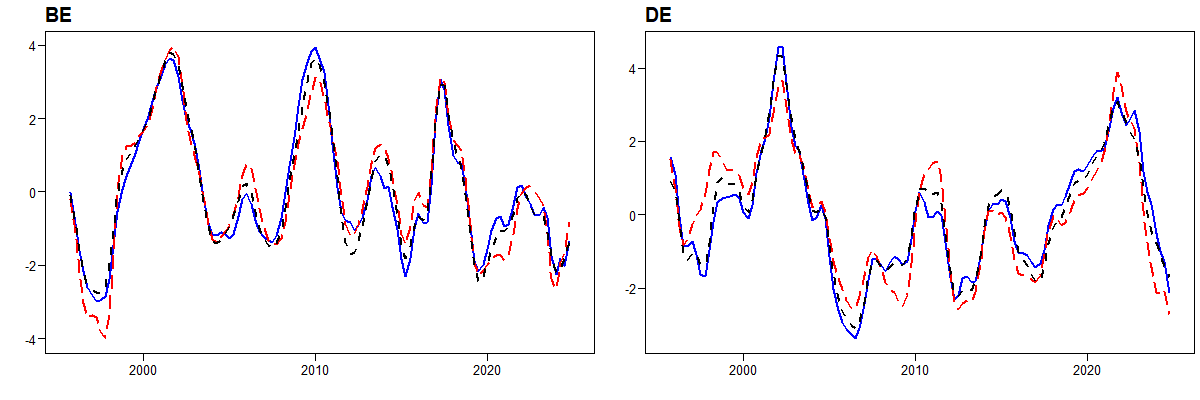
\includegraphics[width=1\linewidth]{TABLES_FIGURES/panel_fc_1_2.png}
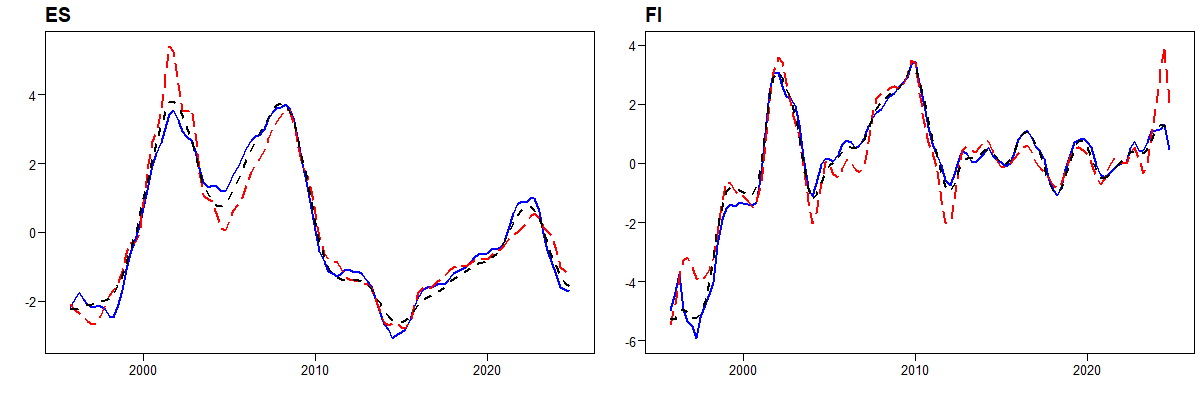
\includegraphics[width=1\linewidth]{TABLES_FIGURES/panel_fc_3_4.png}
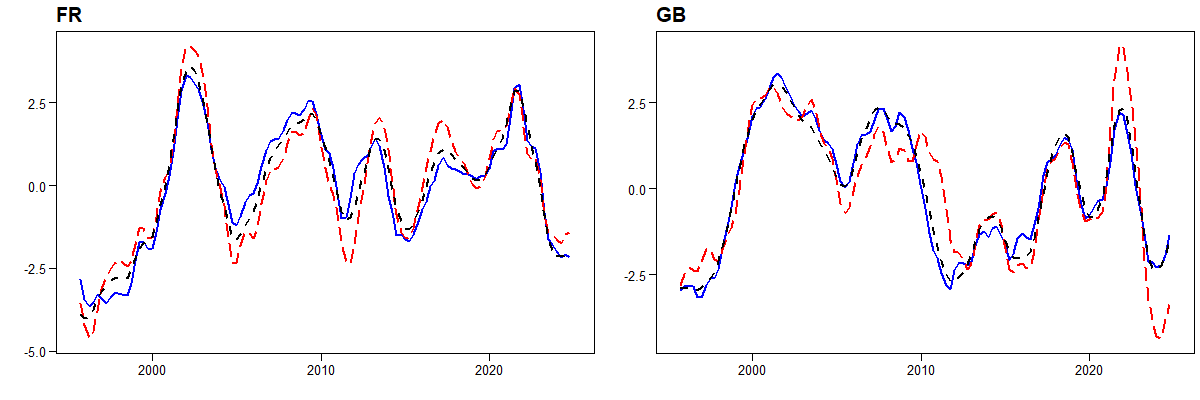
\includegraphics[width=1\linewidth]{TABLES_FIGURES/panel_fc_5_6.png}
\end{figure}
\FloatBarrier
\begin{figure}[h]
    \centering
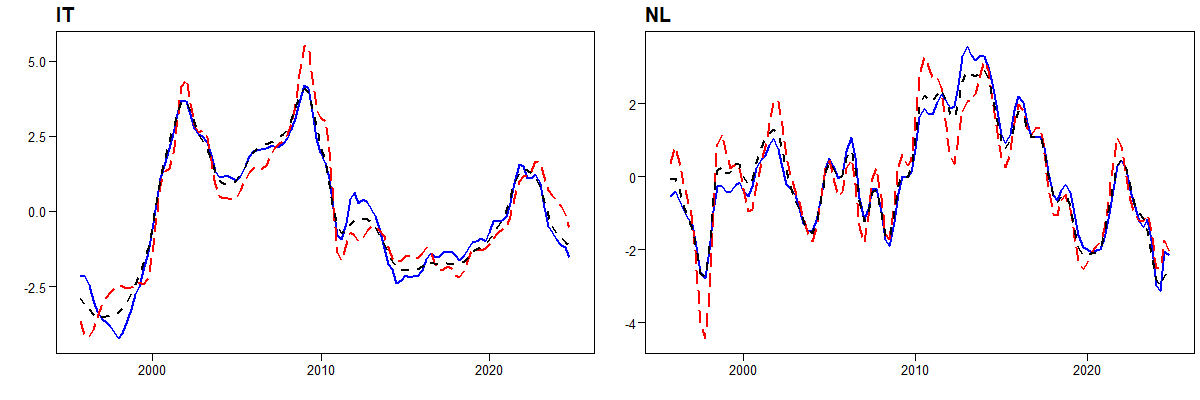
\includegraphics[width=1\linewidth]{TABLES_FIGURES/panel_fc_7_8.png}
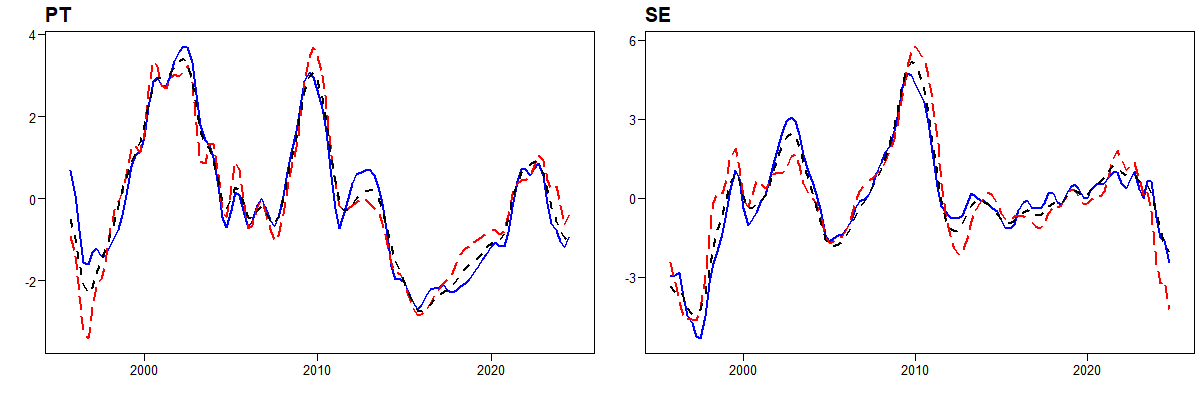
\includegraphics[width=1\linewidth]{TABLES_FIGURES/panel_fc_9_10.png}

\includegraphics[width=5cm]{TABLES_FIGURES/fc_legend.png}
\end{figure}
\FloatBarrier


\section{Financial cycle decomposition \label{AppendixB}}\begin{figure}[h]
    \centering 
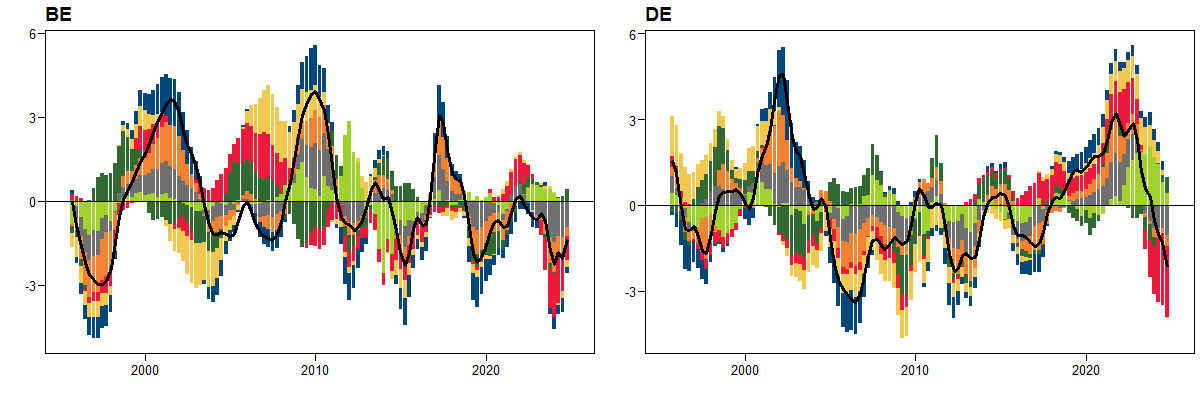
\includegraphics[width=1\linewidth]{TABLES_FIGURES/final_panel_with_legend_1_2.png}
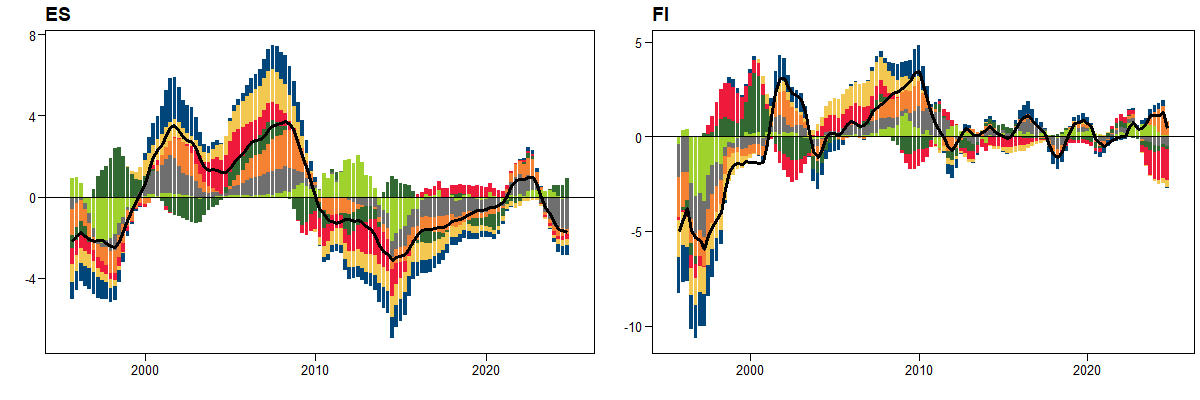
\includegraphics[width=1\linewidth]{TABLES_FIGURES/final_panel_with_legend_3_4.png}
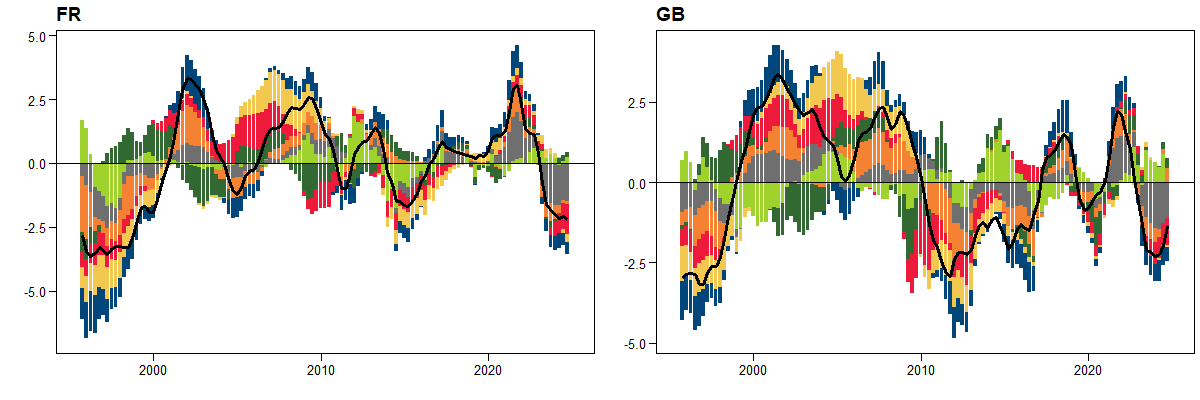
\includegraphics[width=1\linewidth]{TABLES_FIGURES/final_panel_with_legend_5_6.png}
\end{figure}
\FloatBarrier

\begin{figure}[h]
    \centering
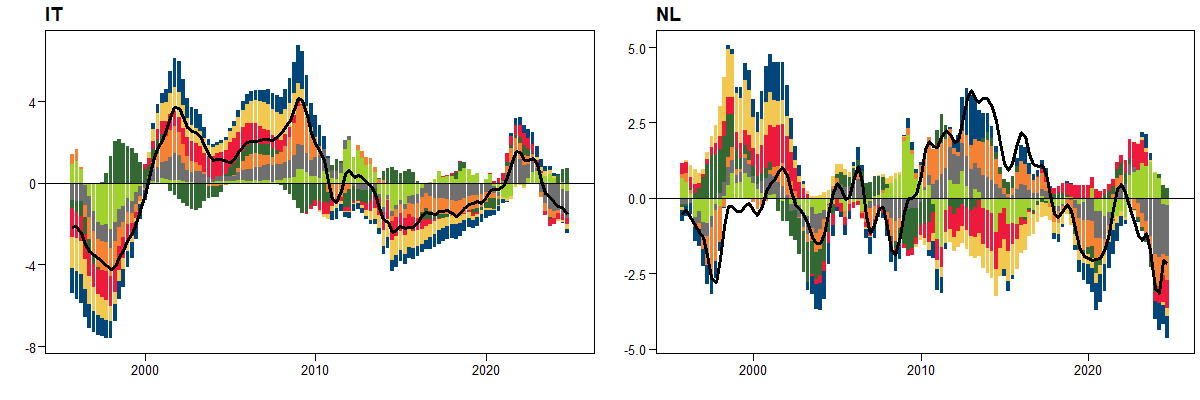
\includegraphics[width=1\linewidth]{TABLES_FIGURES/final_panel_with_legend_7_8.png}
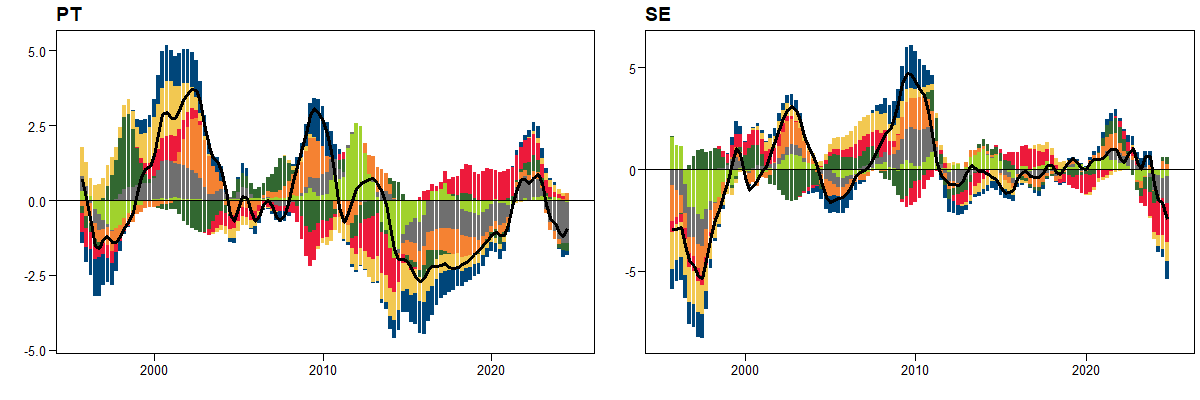
\includegraphics[width=1\linewidth]{TABLES_FIGURES/final_panel_with_legend_9_10.png}
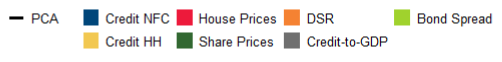
\includegraphics[width=10cm]{TABLES_FIGURES/dec_legend.PNG}
\end{figure}
\FloatBarrier

\section{Factor model confidence intervals \label{AppendixC}}\begin{figure}[h]
    \centering 
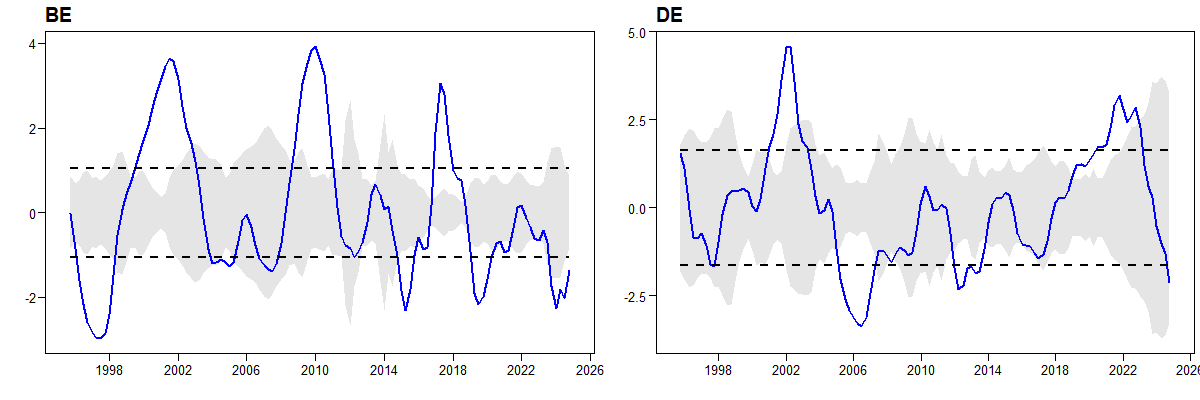
\includegraphics[width=1\linewidth]{TABLES_FIGURES/panel_ci_1_2.png}
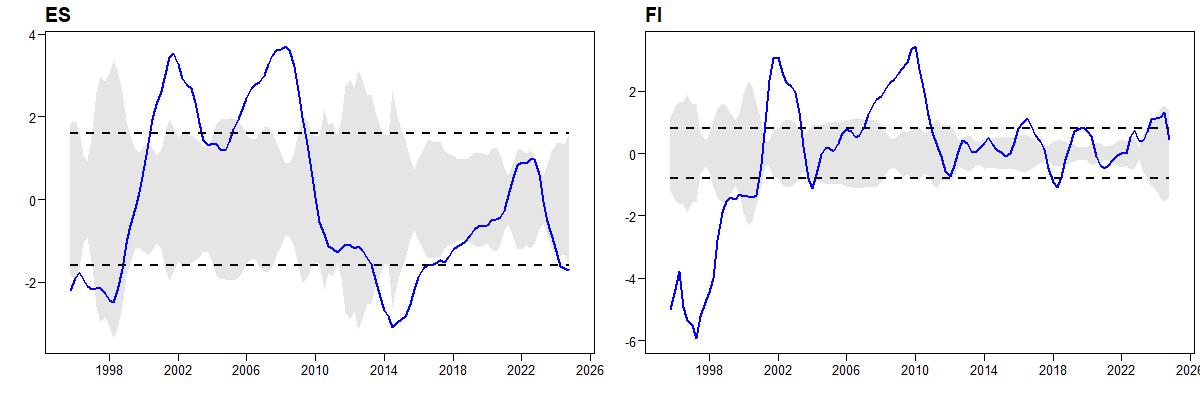
\includegraphics[width=1\linewidth]{TABLES_FIGURES/panel_ci_3_4.png}
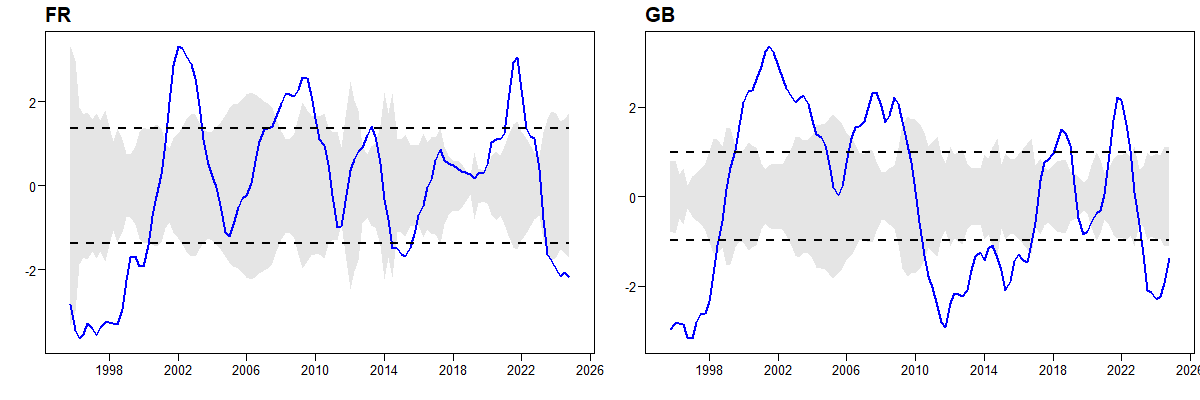
\includegraphics[width=1\linewidth]{TABLES_FIGURES/panel_ci_5_6.png}
\end{figure}
\FloatBarrier

\begin{figure}[h]
    \centering
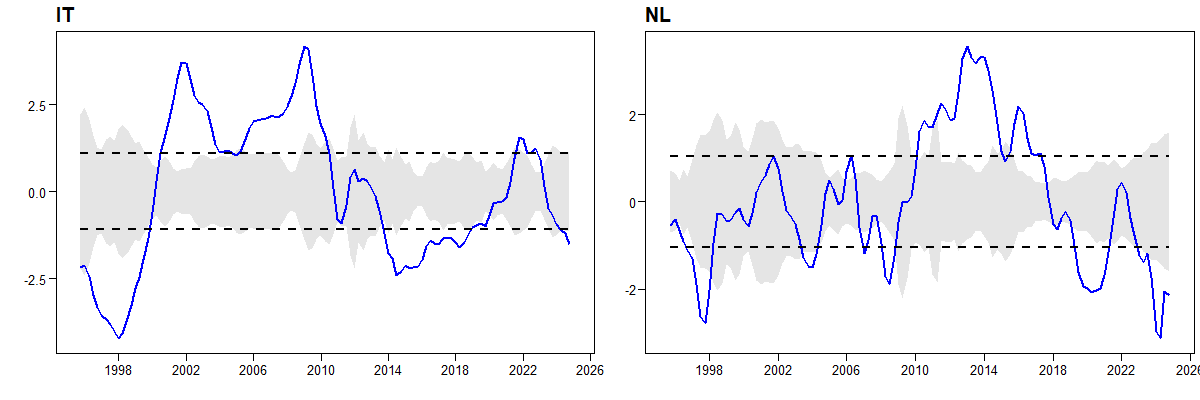
\includegraphics[width=1\linewidth]{TABLES_FIGURES/panel_ci_7_8.png}
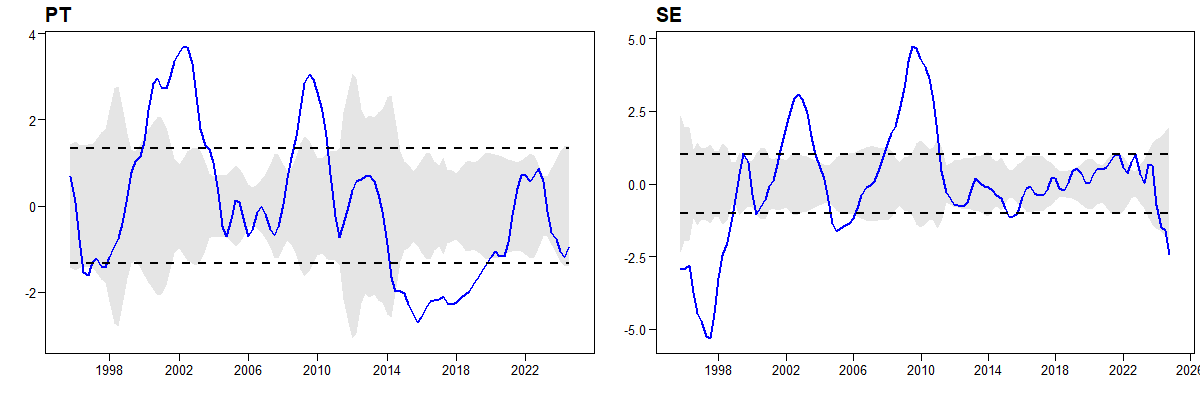
\includegraphics[width=1\linewidth]{TABLES_FIGURES/panel_ci_9_10.png}
\end{figure}
\FloatBarrier




\end{document}
